\section{Methodology Validation}

In the last chapter, the survival probability $S(\tau)$ and the mean
first-passage time has been calculated by solving the heat equation
and approximated by the numerical methods. Lattice Random Walks (LRWs)
and Pearson's Random Walks (PRWs) are implemented in the annulus
image, as shown in \replaced[id=djs, comment={Equation numbers are not mathematical object, thus should not be enclosed by dollar signs.  Also, use the tilde to ensure that the text and figure reference do not become separated at end-of-line breaks.}]{Figure $2.1$}{Figure~2.1}, in Python. This section aims to
validate the research methodology by comparing the estimated survival
functions $S(t)$ of the numerical data with the analytical solutions
$S(\tau)$ where $t$ is the number of steps taken by the particles in
the fixed-time step Monte Carlo simulations and $\tau$ denotes the
unitless time.


\subsection{Statistical Fluctuation Analysis}

Fixed-time step Monte Carlo simulations, LRWs and PRWs, are the
\highlight[id=djs,comment={The word virtual is not correct here.  Do you mean ``numerical''?}]{virtual} representations of the original statistical problem defined in
the continuous-time and continuous-space with numerous inputs and
discrete-time trajectories \highlight[id=djs, comment={This is not correct.  Repeated sampling reduces rather than causes sampling errors.  Also, please define ``over and over'' and ``statistical fluctuation.''}]{sampled randomly over and over again, which
results in the statistical fluctuation.} 

The first kind of error stems from the sampling. As shown in \replaced[id=djs, comment={Removed dollar signs.  Also, it is very important to use references and labels instead of hardcoding figure numbers.  Please look at documentation for more information about how to handle subfigures.  What I did is not quite right.}]{Figure
3.1 (a)}{Figure~\ref{fig:annulus_more_particles}}, the larger sample size in the simulations, the estimated
survival functions will be more precise. LRWs are used to mimic the
continuous-time and continuous-space diffusion process by generating
the discrete random trajectories in the discrete time, which results
in the time-discretization and space-discretization errors. Although
PRWs is a model defined in continuous-time and continuous-space, the
random paths demand much longer time simulation as shown in \replaced[id=djs]{Figure
$3.1 (b)$}{Figure~\label{fig:annulus_finer_steps}}.

\deleted[id=djs,comment={Don't use clearpage.  Instead, allow LaTeX to
    place figures and other ``floating'' objects like
    tables.}]{clearpage}

\begin{figure}
  \begin{subfigure}{0.9\textwidth}
    \centering
    \comment[id=djs]{This figure is illegible because of the overlapping curves and confidence intervals.}    
    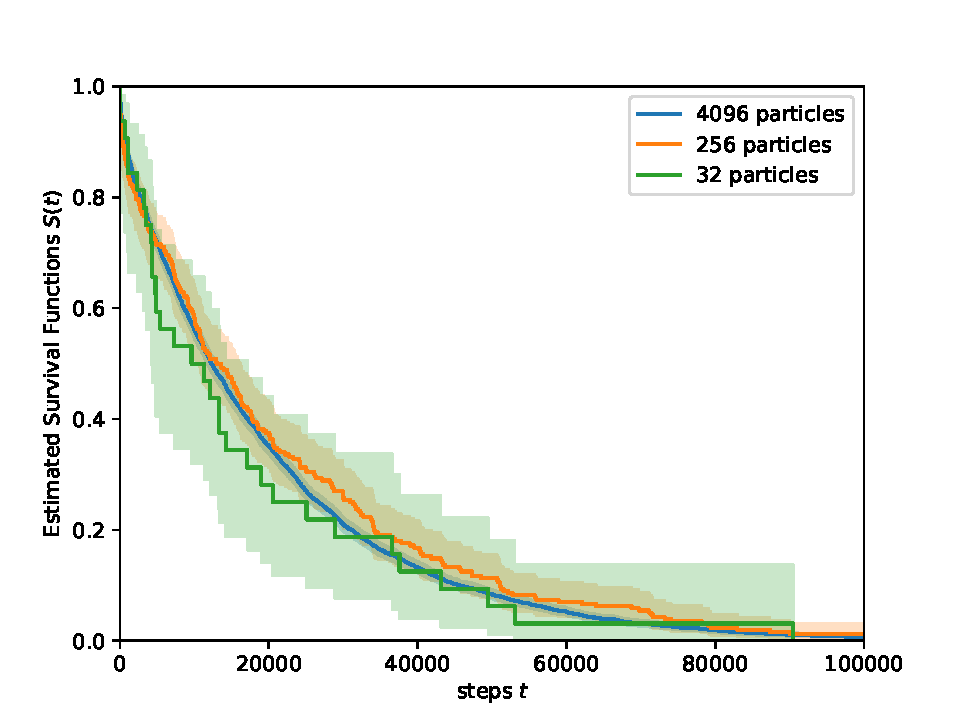
\includegraphics[width=0.8\textwidth]{sampling}
    \caption{As the number of particles increasing, the uncertainty
    of the LRWs simulation are lower since the confidence band of the
    estimated survival function becomes narrower.\label{fig:annulus_more_particles}}
  \end{subfigure}
  \begin{subfigure}{0.9\textwidth}
    \centering
    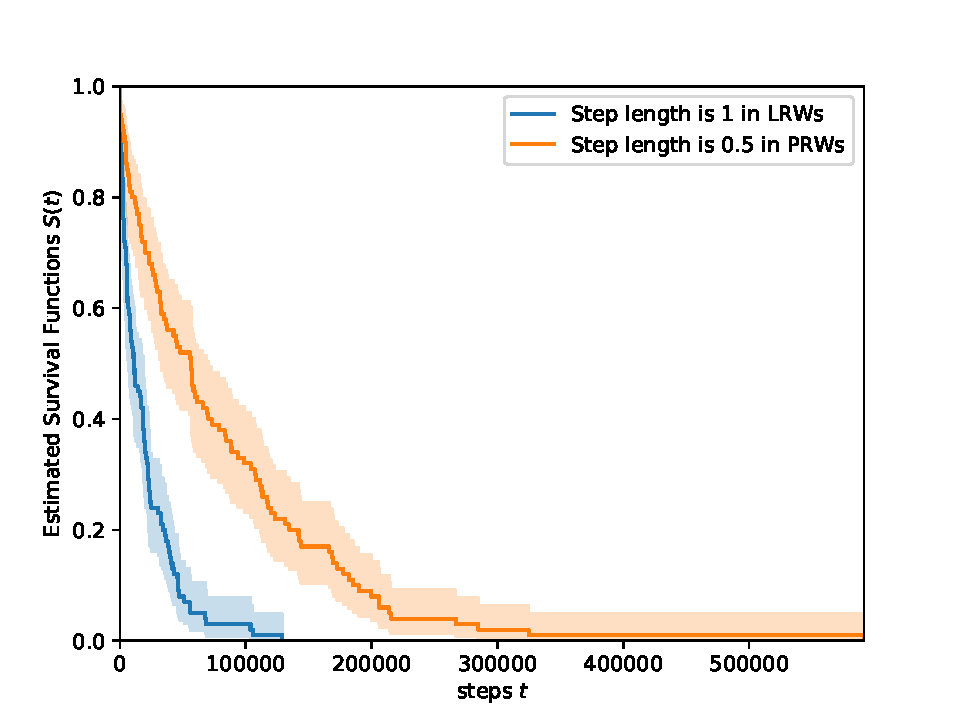
\includegraphics[width=0.8\textwidth]{discretization}
    \caption{When run LRWs and PRWs in the annulus with $100$
      particles, the finer discretization step results in the longer
      simulation time.\label{fig:annulus_finer_steps}}
  \end{subfigure}
  \caption{Estimated survival curves and 95\% confidence intervals for Monte Carlo simulations of partical diffusion on an annulus.\label{fig:lrw_prw_annulus}}
\end{figure}


\subsection{Sample Size Determination and Evaluation}

In the last chapter, two approaches used to determine the appropriate
sample size in the fixed-time step Monte Carlo simulations have been
proposed. One of them is based on inferential statistics
\cite{casella2002statistical}, which infers and estimates the unknown
population parameters from the sample statistics. Another one is
simpler since it does not need any simulations.

\subsubsection{Chebyshev's inequality}

According to LLN \cite{dekking2005modern}, the unknown population mean
first-passage time $\bar X$ can be estimated by sample mean $\bar X_N$
when $N$ is big enough. Chebyshev’s inequality
\cite{chebyshev1867valeurs} is a probabilistic inequality that can be
applied to any probability distribution of a random variable with the
finite expected value and non-zero variance. This inequality provides
an upper bound to the probability that the absolute deviation of a
random variable from its mean will exceed a given threshold.

\begin{figure}
  \begin{subfigure}{0.9\textwidth}
    \centering
    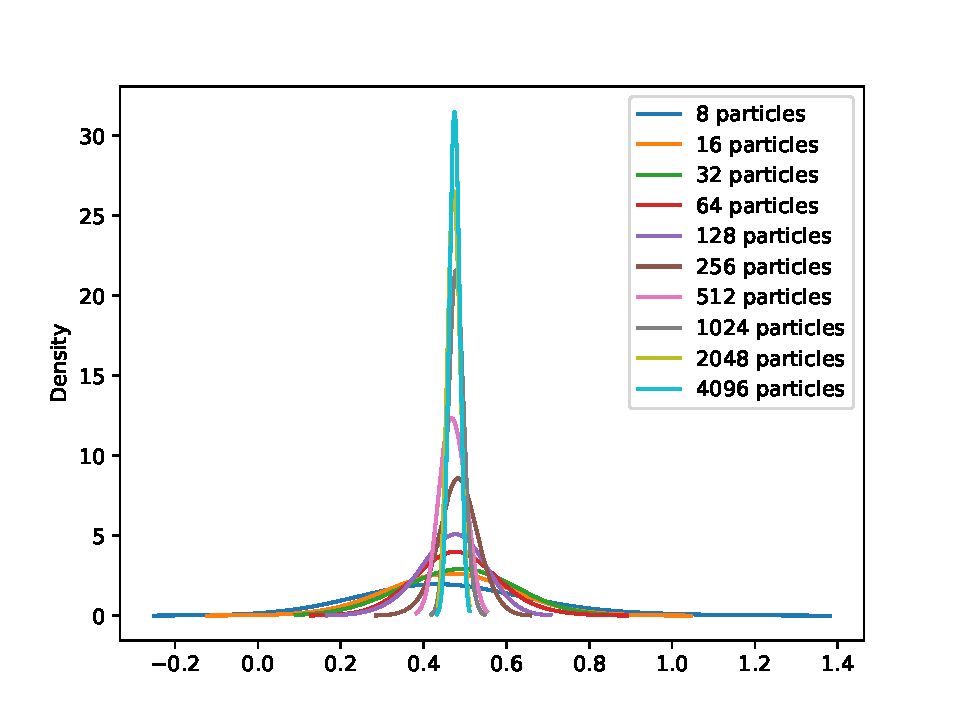
\includegraphics[width=0.9\textwidth]{kde}
    \caption{Running the LRWs in the annulus with $N = 2^i$
      particles and calculating the mean first-passage time $X_N$, where
      $i=3, 4, 5, ..., 12$. For each $N$, replicating the simulation
      $50$ times and recalculating the mean of the mean first-passage
      time $\bar X_{N}$ and the variance $\sigma^2_{N}$. As the sample
      size $N$ increase, the distribution of the sample means $X_N$
      becomes narrower and approximately normal.}
  \end{subfigure}
  \begin{subfigure}{0.9\textwidth}
    \centering
    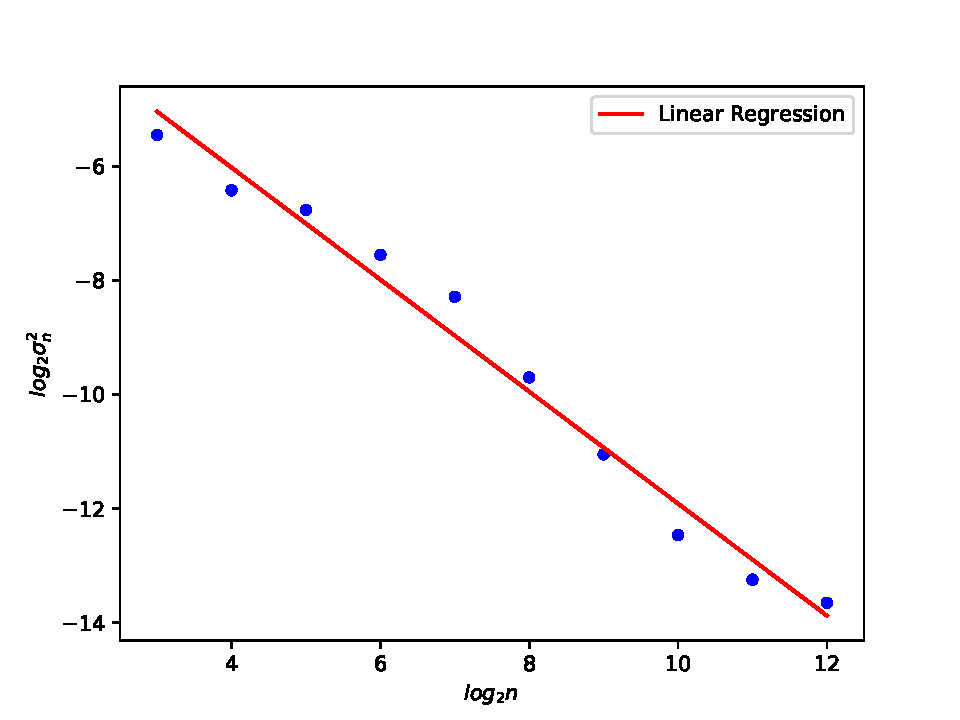
\includegraphics[width=0.8\textwidth]{linear_regression}
    \caption{A fitted linear regression model is used to explore the
      scaling relationship between $log_{2} (\sigma^2_{N})$ and
      $log_{2} N$. $log_{2} (\sigma^2_{N}) \approx b + k log_{2} N$,
      where $k$ and $b$ are the estimated model parameters, slope and
      intercept, respectively.}
  \end{subfigure}
\end{figure}

In the Figure $3.2$, the number of steps $t$ in the numerical
simulations have been converted into the unitless time $\tau$ by the
Eq.$(2.16)$. Thus, given a predesignated error $\epsilon$, the
required number of particles $N$ can be determined by

\begin{equation}
  Pr(|X_{N} - \bar X| \geq \epsilon) = Pr(|X_{N} - \bar X_{N}| \geq
  \epsilon) \leq \frac{\sigma^2_{N}}{\epsilon^2} \approx \frac{2^b
    N^k}{\epsilon^2} = 0.01
\end{equation}

where $\epsilon = 0.01 \bar X$.

The required number of particles in LRWs and PRWs can be estimated by
\highlight[id=djs, comment={Never hard code equation numbers!}]{Eq.(3.3)}, which is

\begin{equation}
  N \geq (\frac{0.01 \epsilon^2}{2^b})^{\frac{1}{k}} \approx 1338643
\end{equation}

where $\epsilon \approx 0.004744$, $b \approx -2.088495$, and $k
\approx -0.982400$. Therefore, the number of particles should be at
least $1338643$ to make sure that there is no more than $1\%$ chance
of $X_N$ to be outside $[0.46865856, 0.47812641]$.


\begin{figure}
  \begin{subfigure}{0.9\textwidth}
    \centering
    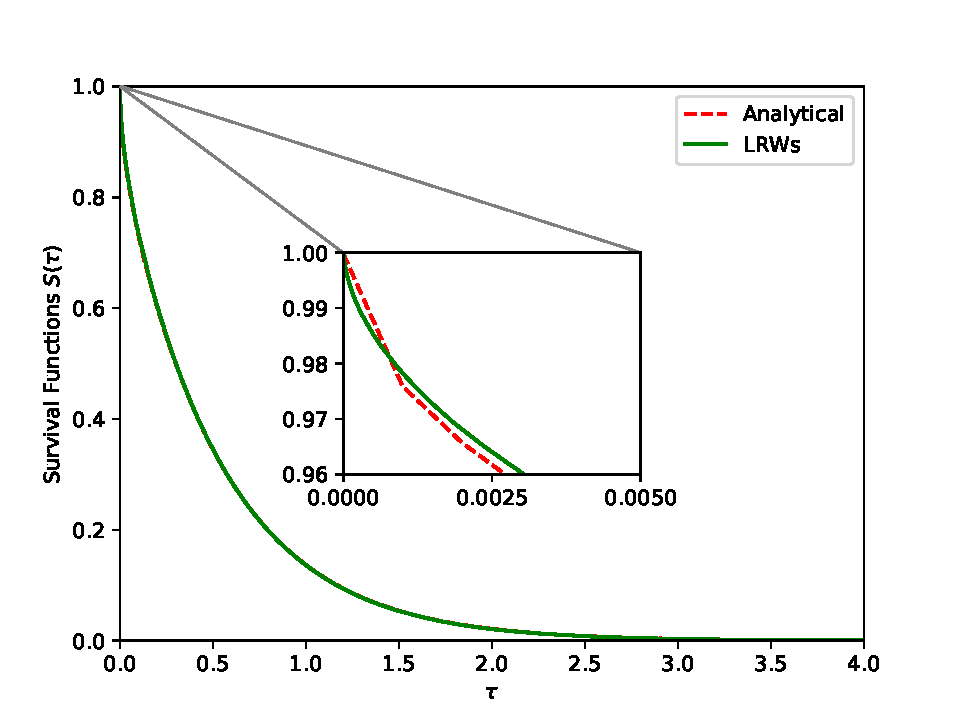
\includegraphics[width=0.8\textwidth]{LRWscheb}
    \caption{Survival curve for LRW.\label{fig:LRW_survival}}
  \end{subfigure}
  \begin{subfigure}{0.9\textwidth}
    \centering
    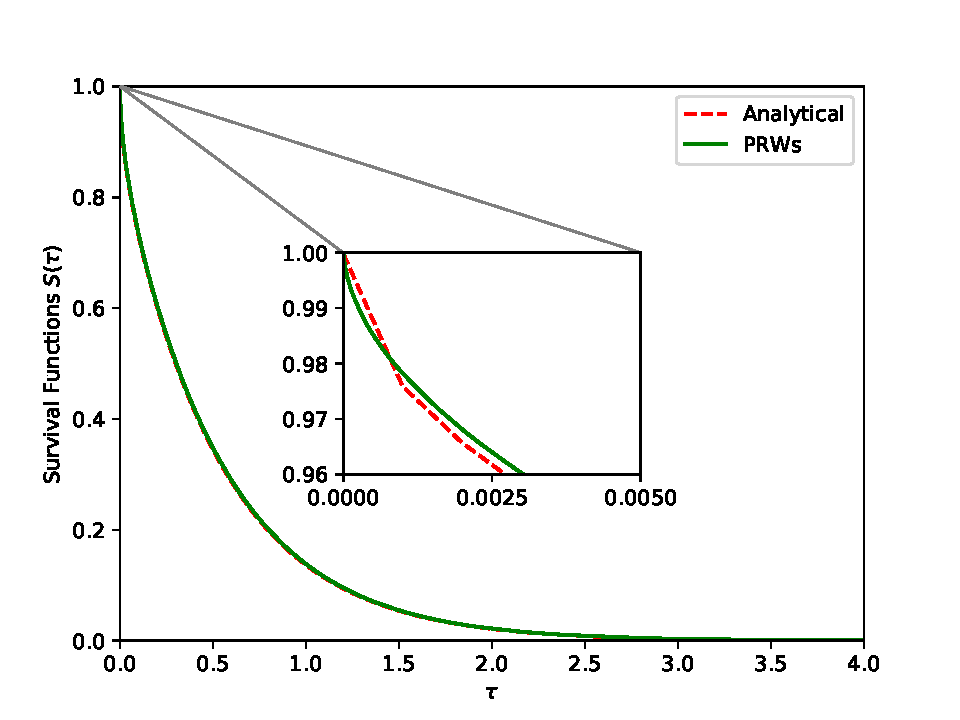
\includegraphics[width=0.8\textwidth]{PRWscheb}
    \caption{Survival curve for PRW.\label{fig:PRW_survival}}
  \end{subfigure}
  \caption{Running PRWs and LRWs in the annulus with $1338643$
    particles determined by the ???? illustrating
    that the short and long time asypototic behaviors of the estimated
    survival functions of particles undergoing LRWs and PRWs
    are consistent with the analytical result in Equation ????.}
\end{figure}

\begin{table}
  \centering
  \begin{tabular}{|c|c|c|}\hline
    Test Methods (standard nonparametric) & Statistics & P Values \\
    \hline
    Logrank & 0.017679 & 0.894223 \\
    \hline
    Fleming-Harrington & 0.742536 & 0.388850 \\
    \hline
    Gehan-Breslow & 0.742536 & 0.388850 \\
    \hline
    Tarone-Ware & 0.499418 & 0.479756 \\
    \hline
  \end{tabular}
  \caption{The estimated survival function of $1338643$ particles in
    the LRWs is statistically similar to the analytical survival
    function. NEED LABEL HERE}
\end{table}

\begin{table}
  \centering
  \begin{tabular}{|c|c|c|}\hline
    Test Methods (standard nonparametric) & Statistics & P Values \\
    \hline
    Logrank & 0.039142 & 0.843168 \\
    \hline
    Fleming-Harrington & 0.083388 & 0.772757 \\
    \hline
    Gehan-Breslow & 0.083388 & 0.772757 \\
    \hline
    Tarone-Ware & 0.010582 & 0.918069 \\
    \hline
  \end{tabular}
  \caption{The estimated survival function of PRWs, which has
    $1338643$ particles with step length $0.5$, is not statistically
    different from the analytical survival function. NEED LABEL HERE}
\end{table}

From the visualized comparison in Figure $3.3$ and the results of the
two-sample statistical tests, the fixed-step Monte Carlo simulations'
results converge to the analytical outcomes. Therefore, the integral
of the solutions of heat equations can be approximated by the Monte
Carlo simulations without calculating manually. As mentioned in the
last chapter, the integral, $S(\tau)$, indicates the annulus'
geometrical information. Therefore, the fixed-time step Monte Carlo
simulation can describe the shape of an object without using the
rulers. However, the number of particles in the numerical simulations
estimated by Eq.$(3.1)$ is abundant, which causes a high computational
cost because each random trajectories of each particle are simulated
in LRWs and PRWs till they reach the inner boundary of the annulus. 


\subsubsection{Dvoretzky–Kiefer–Wolfowitz (DKW) inequality}

Chebyshev's inequality can be applied to any probability distribution,
but it is also weaker than other inequalities. DKW inequality is more
efficient since the confidence band is generated without running any
simulations. For example, let $F(\tau)$ be the true cumulative
distribution function (CDF) of the first passage time, a continuous unitless
random variable on the interval $[0, \infty]$. $F(\tau)$ has a
relationship with $S(\tau)$, which is

\begin{equation}
  F(\tau) = 1 - S(\tau)
\end{equation}

The true CDF is known by Eq.$(3.3)$, which can also be approximated
numerically. A simple example of generating the CDF-based confidence
bounds by DKW inequality is shown in Fig.$3.4$. The empirical
distribution function $F_{256}(\tau)$ is estimated by the lifeline
module in Python \cite{davidson2019lifelines}. Thus, the interval
$\varepsilon$ contains the entire $F(\tau)$ with the probability
$95\%$ can be calculated by Eq.$(2.20)$

\begin{equation}
  \varepsilon = \sqrt{\frac{\ln{\frac{2}{0.05}}}{2* 256}} \approx 0.084881
\end{equation}

\begin{figure}
  \centering
  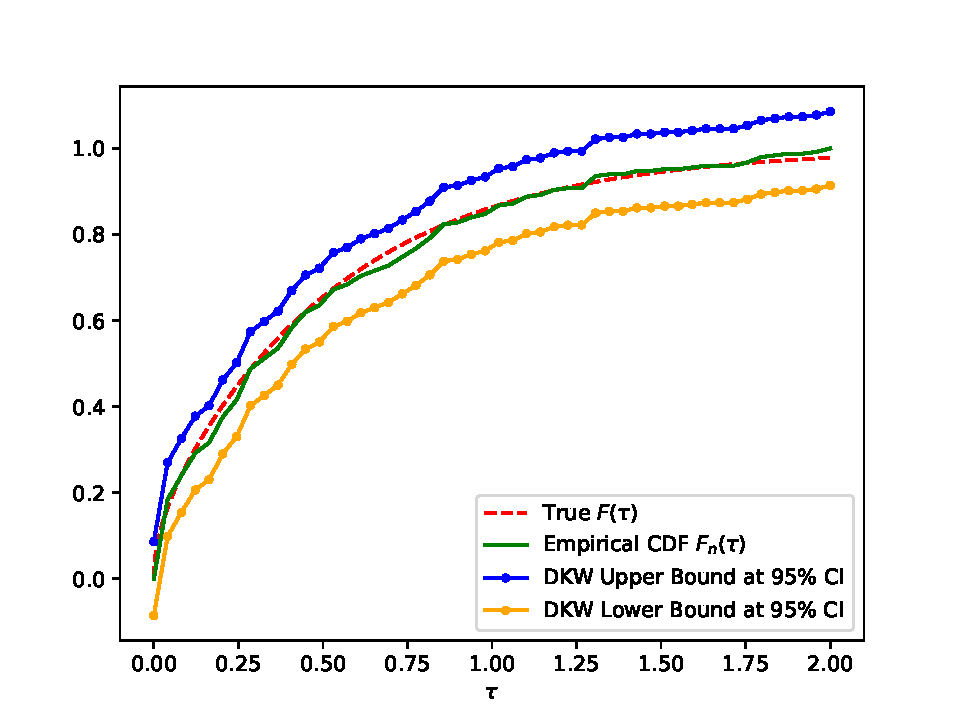
\includegraphics[width=0.8\textwidth]{dkw_comfidence_band_demo}
  \caption{The simultaneous band around $F_{256}(\tau)$ with interval
    $0.084881$ calculate by Eq.$(3.4)$ encompasses the entire $F(x)$
    at $95\%$ confidence level. NEED LABEL HERE}
\end{figure}



Moreover, the sample size estimated by DKW inequality Eq.$(2.20)$ does
not depend on the geometries or the kind of simulations because the
simultaneous confidence bounds always contain the true cumulative
distribution at a specific confidence level. For instance, assume the
probability, that the maximum distance between $F_N(\tau)$ and
$F(\tau)$ is bigger than $0.005$, is smaller than $0.01$, the minimum
required number of particles should meet the inequality

\begin{equation}
  Pr(\sup_{x \in \mathbb{R}} |F_{N}(\tau) - F(\tau)| > 0.005) \leq 2e^{-2N0.005^2} = 0.01
\end{equation}

Thus

\begin{equation}
  N \geq \frac{\ln(\frac{0.01}{2})}{-2 \times 0.005^2} \approx
  105966
\end{equation}


\begin{figure}
  \begin{subfigure}{0.9\textwidth}
    \centering
    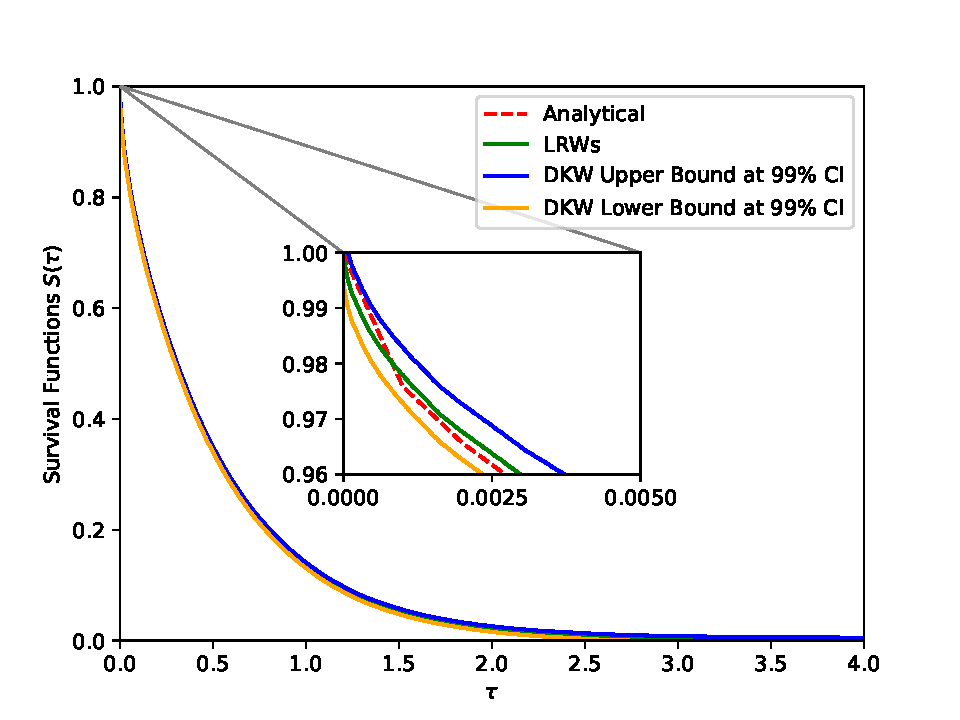
\includegraphics[width=0.8\textwidth]{LRWsdkw}
    \caption{Need a caption here, and label!}
  \end{subfigure}
  \begin{subfigure}{0.9\textwidth}
    \centering
    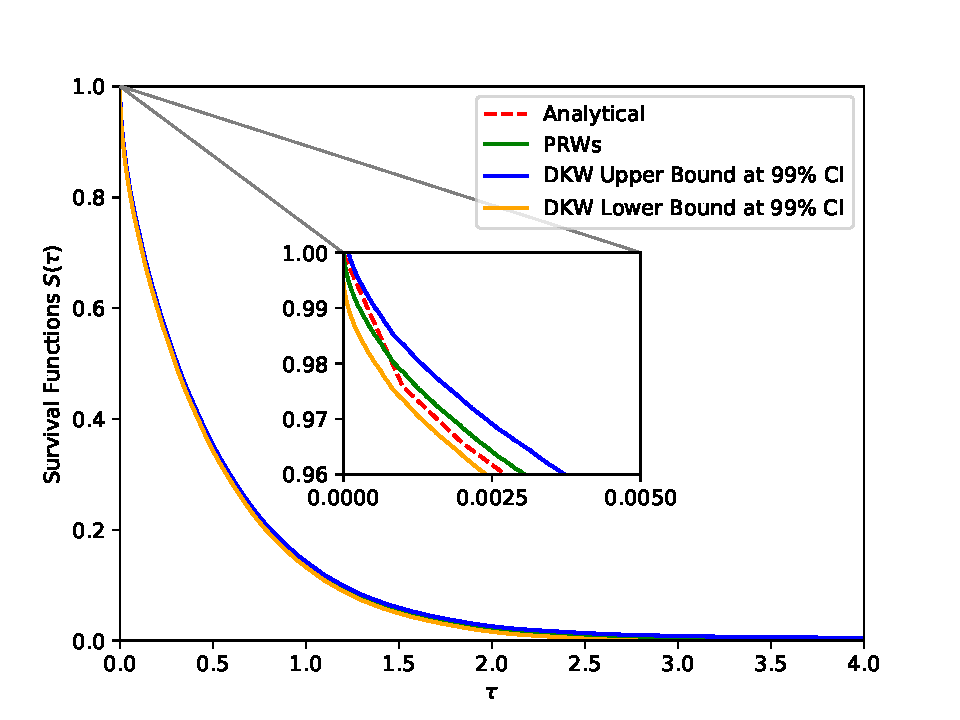
\includegraphics[width=0.8\textwidth]{PRWsdkw}
    \caption{Need caption and label here too.}
  \end{subfigure}
  \caption{PRWs and LRWs are implemented in the annulus with $105966$
    particles determined by the Eq.$(3.6)$. (a) and (b) show that the
    simultaneous confidence bands of estimated survival function with
    the interval $0.005$ contain the entire analytical $S(\tau)$ at
    $99 \%$ confidence level. NEED LABEL HERE}
\end{figure}

\begin{table}
  \centering
  \begin{tabular}{|c|c|c|}\hline
    Test Methods (standard nonparametric) & Statistics & P Values \\
    \hline
    Logrank & 1.532224 & 0.215779 \\
    \hline
    Fleming-Harrington & 1.630358 & 0.201654 \\
    \hline
    Gehan-Breslow & 1.630358 & 0.201654 \\
    \hline
    Tarone-Ware & 1.619530 & 0.203157 \\
    \hline
  \end{tabular}
  \caption{The estimated survival function of $105966$ particles in
    the LRWs is not statistically different to the analytical survival
    function. NEED LABEL HERE}
\end{table}


\begin{table}
  \centering
  \begin{tabular}{|c|c|c|}\hline
    Test Methods (standard nonparametric) & Statistics & P Values \\
    \hline
    Logrank & 2.645624 & 0.103835 \\
    \hline
    Fleming-Harrington & 1.473674 & 0.224767 \\
    \hline
    Gehan-Breslow & 1.473674 & 0.224767 \\
    \hline
    Tarone-Ware & 1.986810 & 0.158675 \\
    \hline
  \end{tabular}
  \caption{The estimated survival function of PRWs, which has
    $105966$ particles with step length $0.5$, is statistically
    similar to the analytical survival function. NEED LABEL HERE}
\end{table}


\subsection{Conclusion}


Instead of calculating the asymptotic expansion of the heat content
manually as $\tau \rightarrow 0^+$, the total heat energy $\beta$
\cite{gilkey1994heat} for time $\tau > 0$ can be approximated by the
fixed-time step Monte Carlo simulations for describing the full-scale
geometrical features of the annulus. Moreover, the required number of
particles in the simulations determined by the DKW inequality is much
smaller than the superabundant value estimated by Chebyshev’s
inequality. 
